\chapter{Dane testowe}\label{chap:testdata}
W celu przeprowadzenia szczegółowej analizy efektywności algorytmów optymalizujących zakup licencji w sieciach społecznościowych niezbędne było wykorzystanie różnorodnych danych testowych. Posłużyły do tego syntetycznie generowane grafy losowe oraz rzeczywiste fragmenty sieci społecznościowej. Pierwsza grupa stanowi kontrolowany zbiór danych sztucznych, pozwalający na symulowanie różnych scenariuszy topologicznych i analizę wpływu struktury sieci na działanie algorytmów. Druga grupa to rzeczywiste ego-sieci z platformy Facebook, umożliwiające weryfikację metod na prawdziwych danych społecznościowych.

Niniejszy rozdział koncentruje się na charakterystyce wykorzystanych danych, natomiast ich praktyczne zastosowanie zostanie szczegółowo przedstawione w części poświęconej opisowi przeprowadzonych eksperymentów.

\section{Grafy syntetyczne}

Do generowania danych syntetycznych wykorzystano trzy standardowe modele grafów: Erd\H{o}s--Rényi (ER), Barabási--Albert (BA) oraz Watts--Strogatz (WS).
W eksperymentach wykorzystywano kilka odrębnych konfiguracji rozmiaru w zależności od scenariusza eksperymentalnego:
\begin{itemize}
  \item \textbf{Benchmark statyczny} (rozdz.\,\ref{chap:experiments}) obejmował grafy o $n \in \{20, 40, 60, 80, 100, 120, 140, 160, 180,\\200, 300, 600, 1000\}$, generowane po trzy próbki na rozmiar.
  \item \textbf{Symulacje dynamiczne} (rozdz.\,\ref{chap:dynamic}) korzystały z mniejszego wachlarza wielkości: dla mutacji syntetycznych $n \in \{20, 40, 80, 160, 320, 640\}$, natomiast warianty realistyczne (pref\_triadic, pref\_pref, rand\_rewire) operowały odpowiednio na zestawach $\{40, 80, 160, 320\}$ oraz $\{40, 80, 160, 320, 640\}$.
  \item \textbf{Rozszerzenia taryfowe} (rozdz.\ref{chap:extensions}) w wariancie statycznym analizowano na rozmiarach $n \in \{20, 50, 100, 200\}$, natomiast część dynamiczna korzystała z $n \in \{40, 80, 160\}$ przy krótszym horyzoncie czasowym.
\end{itemize}


\subsection{Model Erdős--Rényi - klasyczne grafy losowe}
Pierwszym rozważanym modelem jest klasyczny losowy graf Erdős--Rényi (ER) zaproponowany przez Erd\H{o}s'a i Rényi'ego w 1959 roku \cite{ErdosRenyi1960}. W modelu tym rozpatruje się zbiór $n$ wierzchołków, a każda z $\binom{n}{2}$ potencjalnych krawędzi pojawia się niezależnie z prawdopodobieństwem $p$. Parametrami modelu są więc $n$ oraz $p$. W używanej implementacji zaadaptowano właśnie ten wariant $G(n,p)$, który prezentuje się w sposób przedstawiony na rys. \ref{fig:ER}.

\begin{figure}[h]
    \centering
    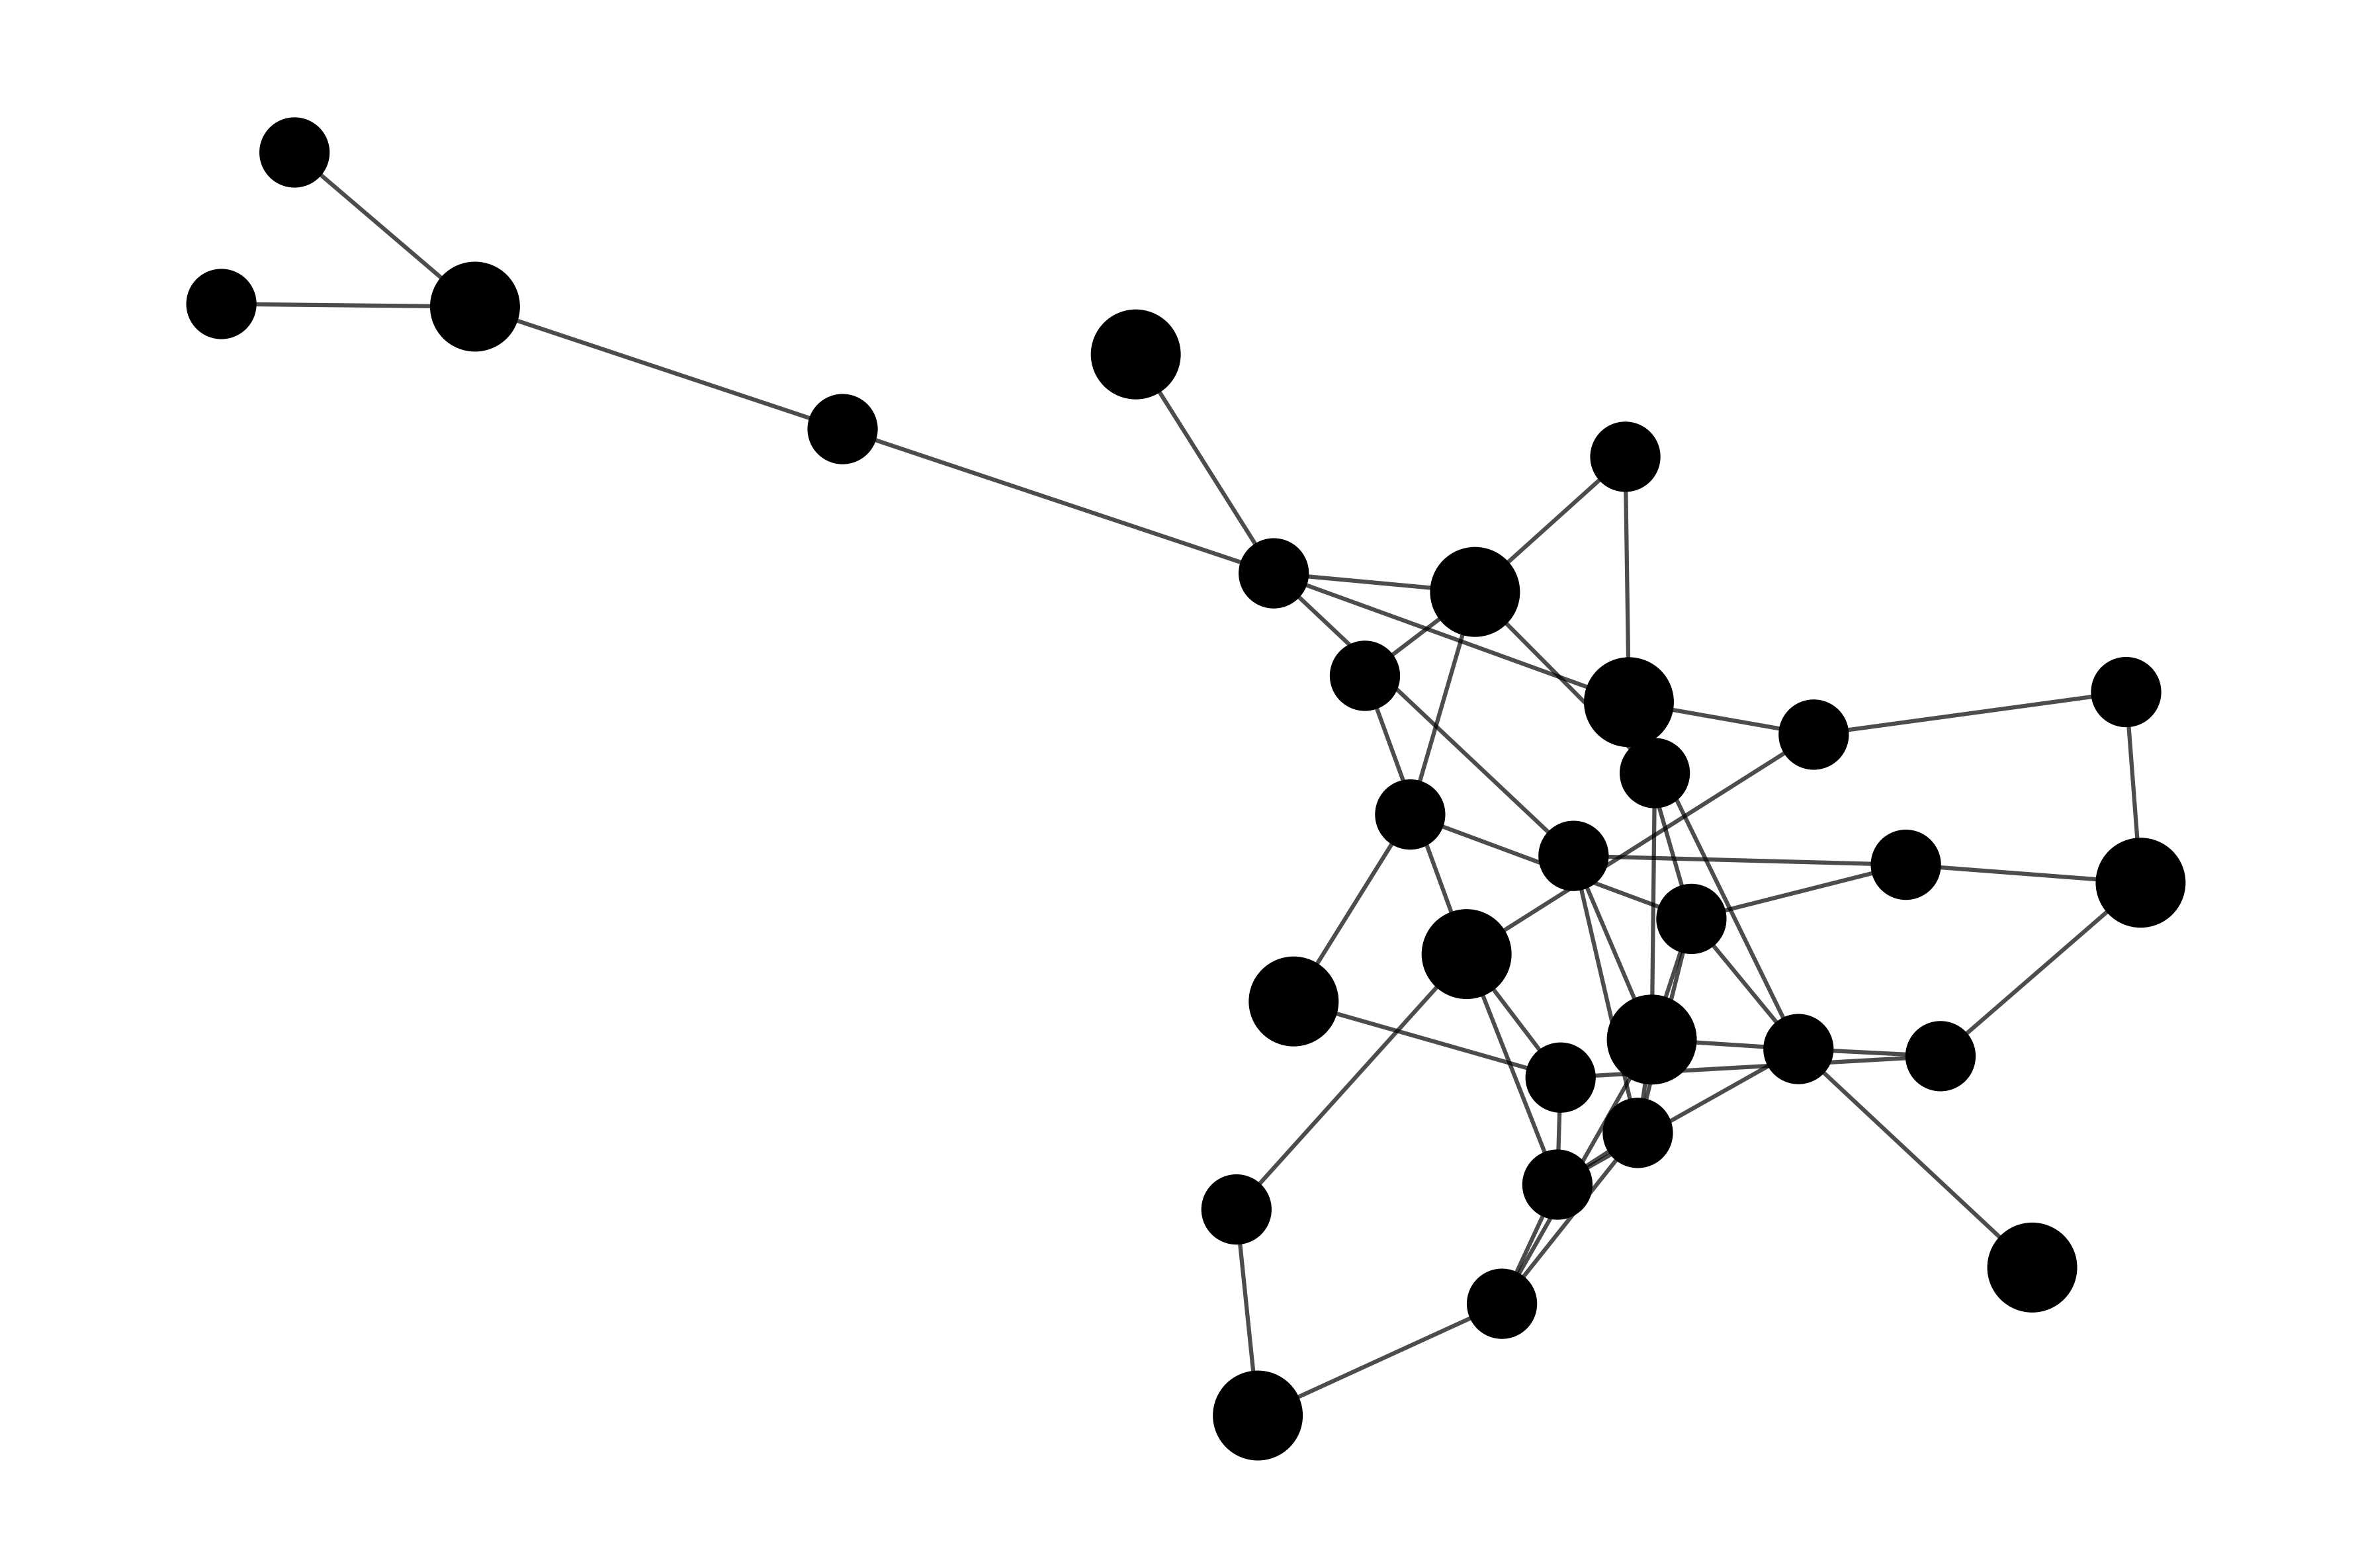
\includegraphics[width=0.6\textwidth]{assets/test_data/random.png}
    \caption{Przykładowa realizacja grafu Erdős--Rényi}
    \label{fig:ER}
\end{figure}

Model ER stanowi istotny punkt odniesienia jako najprostszy model sieci pozbawiony struktury społecznościowej. Motywacją uwzględnienia go w testach jest możliwość porównania działania algorytmów na zupełnie przypadkowych sieciach z ich działaniem na bardziej uporządkowanych grafach takich jak grafy skalowane, małego świata oraz rzeczywiste. Choć prawdziwe sieci społecznościowe odbiegają od założeń pełnej losowości, mają zwykle wyższy poziom klasteryzacji węzłów i nierównomierny rozkład stopni, to jednak model $G(n, p)$ stanowi istotną podstawę porównawczą.

Z punktu widzenia właściwości, grafy ER cechują się stosunkowo niskim średnim współczynnikiem klasteryzacji.
Współczynnik klasteryzacji mierzy, w jakim stopniu sąsiedzi danego wierzchołka są ze sobą połączeni. 
Dokładniej, oblicza się go jako stosunek liczby krawędzi faktycznie istniejących między sąsiadami wierzchołka do liczby wszystkich możliwych krawędzi między tymi sąsiadami. 
Średni współczynnik klasteryzacji dla całego grafu definiuje się jako średnią arytmetyczną wartości współczynników klasteryzacji po wszystkich wierzchołkach.
Oczekiwana wartość współczynnika klasteryzacji jest równa $p$ dla wystarczająco dużego $n$, a dla dostatecznie dużego $p$ istnieje możliwość powstania jednej gigantycznej składowej spójności.
Istnieje znana granica perkolacji, gdy $p>\frac{\ln n}{n}$, graf ER jest z dużym prawdopodobieństwem spójny - poniżej tego progu sieć rozpada się na wiele składowych \cite{ErdosRenyi1960}. Gęstość grafu, rozumiana jako odsetek istniejących krawędzi w stosunku do wszystkich możliwych, wynosi w tym modelu w przybliżeniu $p$. Przykładowo, dla $p=0.1$ graf będzie miał ok. 10\% maksymalnej liczby krawędzi. Rozkład stopni w modelu ER ma charakter dwumianowy, przy czym zbiega do rozkładu Poissona przy $n\to\infty$. Oznacza to, że w grafach tych nie występują węzły o niezwykle wysokich stopniach (tzw. huby), które są charakterystyczne dla wielu rzeczywistych sieci społecznościowych. W konsekwencji model ER nie oddaje wielu kluczowych właściwości takich sieci - stanowi jednak użyteczny model kontrolny, pozbawiony zjawisk typu mały świat czy skalowość, dzięki czemu można wyraźnie uwypuklić wpływ tych cech w innych modelach.


\subsection{Model Barabási--Albert - sieci bezskalowe}
Drugim wykorzystanym generatorem jest model Barabási--Albert (BA), wprowadzony przez Barabási'ego i Alberta w 1999 roku \cite{barabasi1999emergence}. Model BA pozwala generować grafy o strukturze bezskalowej, których rozkład stopni wierzchołków ma rozkład wykładniczy. Tego typu sieci charakteryzują się istnieniem niewielkiej liczby wierzchołków o bardzo wysokim stopniu (tzw. hubów) oraz wielu wierzchołków o małym stopniu - jest to cecha obserwowana w wielu rzeczywistych sieciach, w tym społecznościowych. Dla ilustracji, na rys.~\ref{fig:BA} przedstawiono przykładową realizację grafu BA, w której wyraźnie widoczne są huby. W przypadku sieci społecznościowych odnosi się to do tego, że niektórzy użytkownicy mogą mieć tysiące znajomych/obserwujących, podczas gdy większość ma ich kilkadziesiąt lub mniej.

\begin{figure}[h]
    \centering
    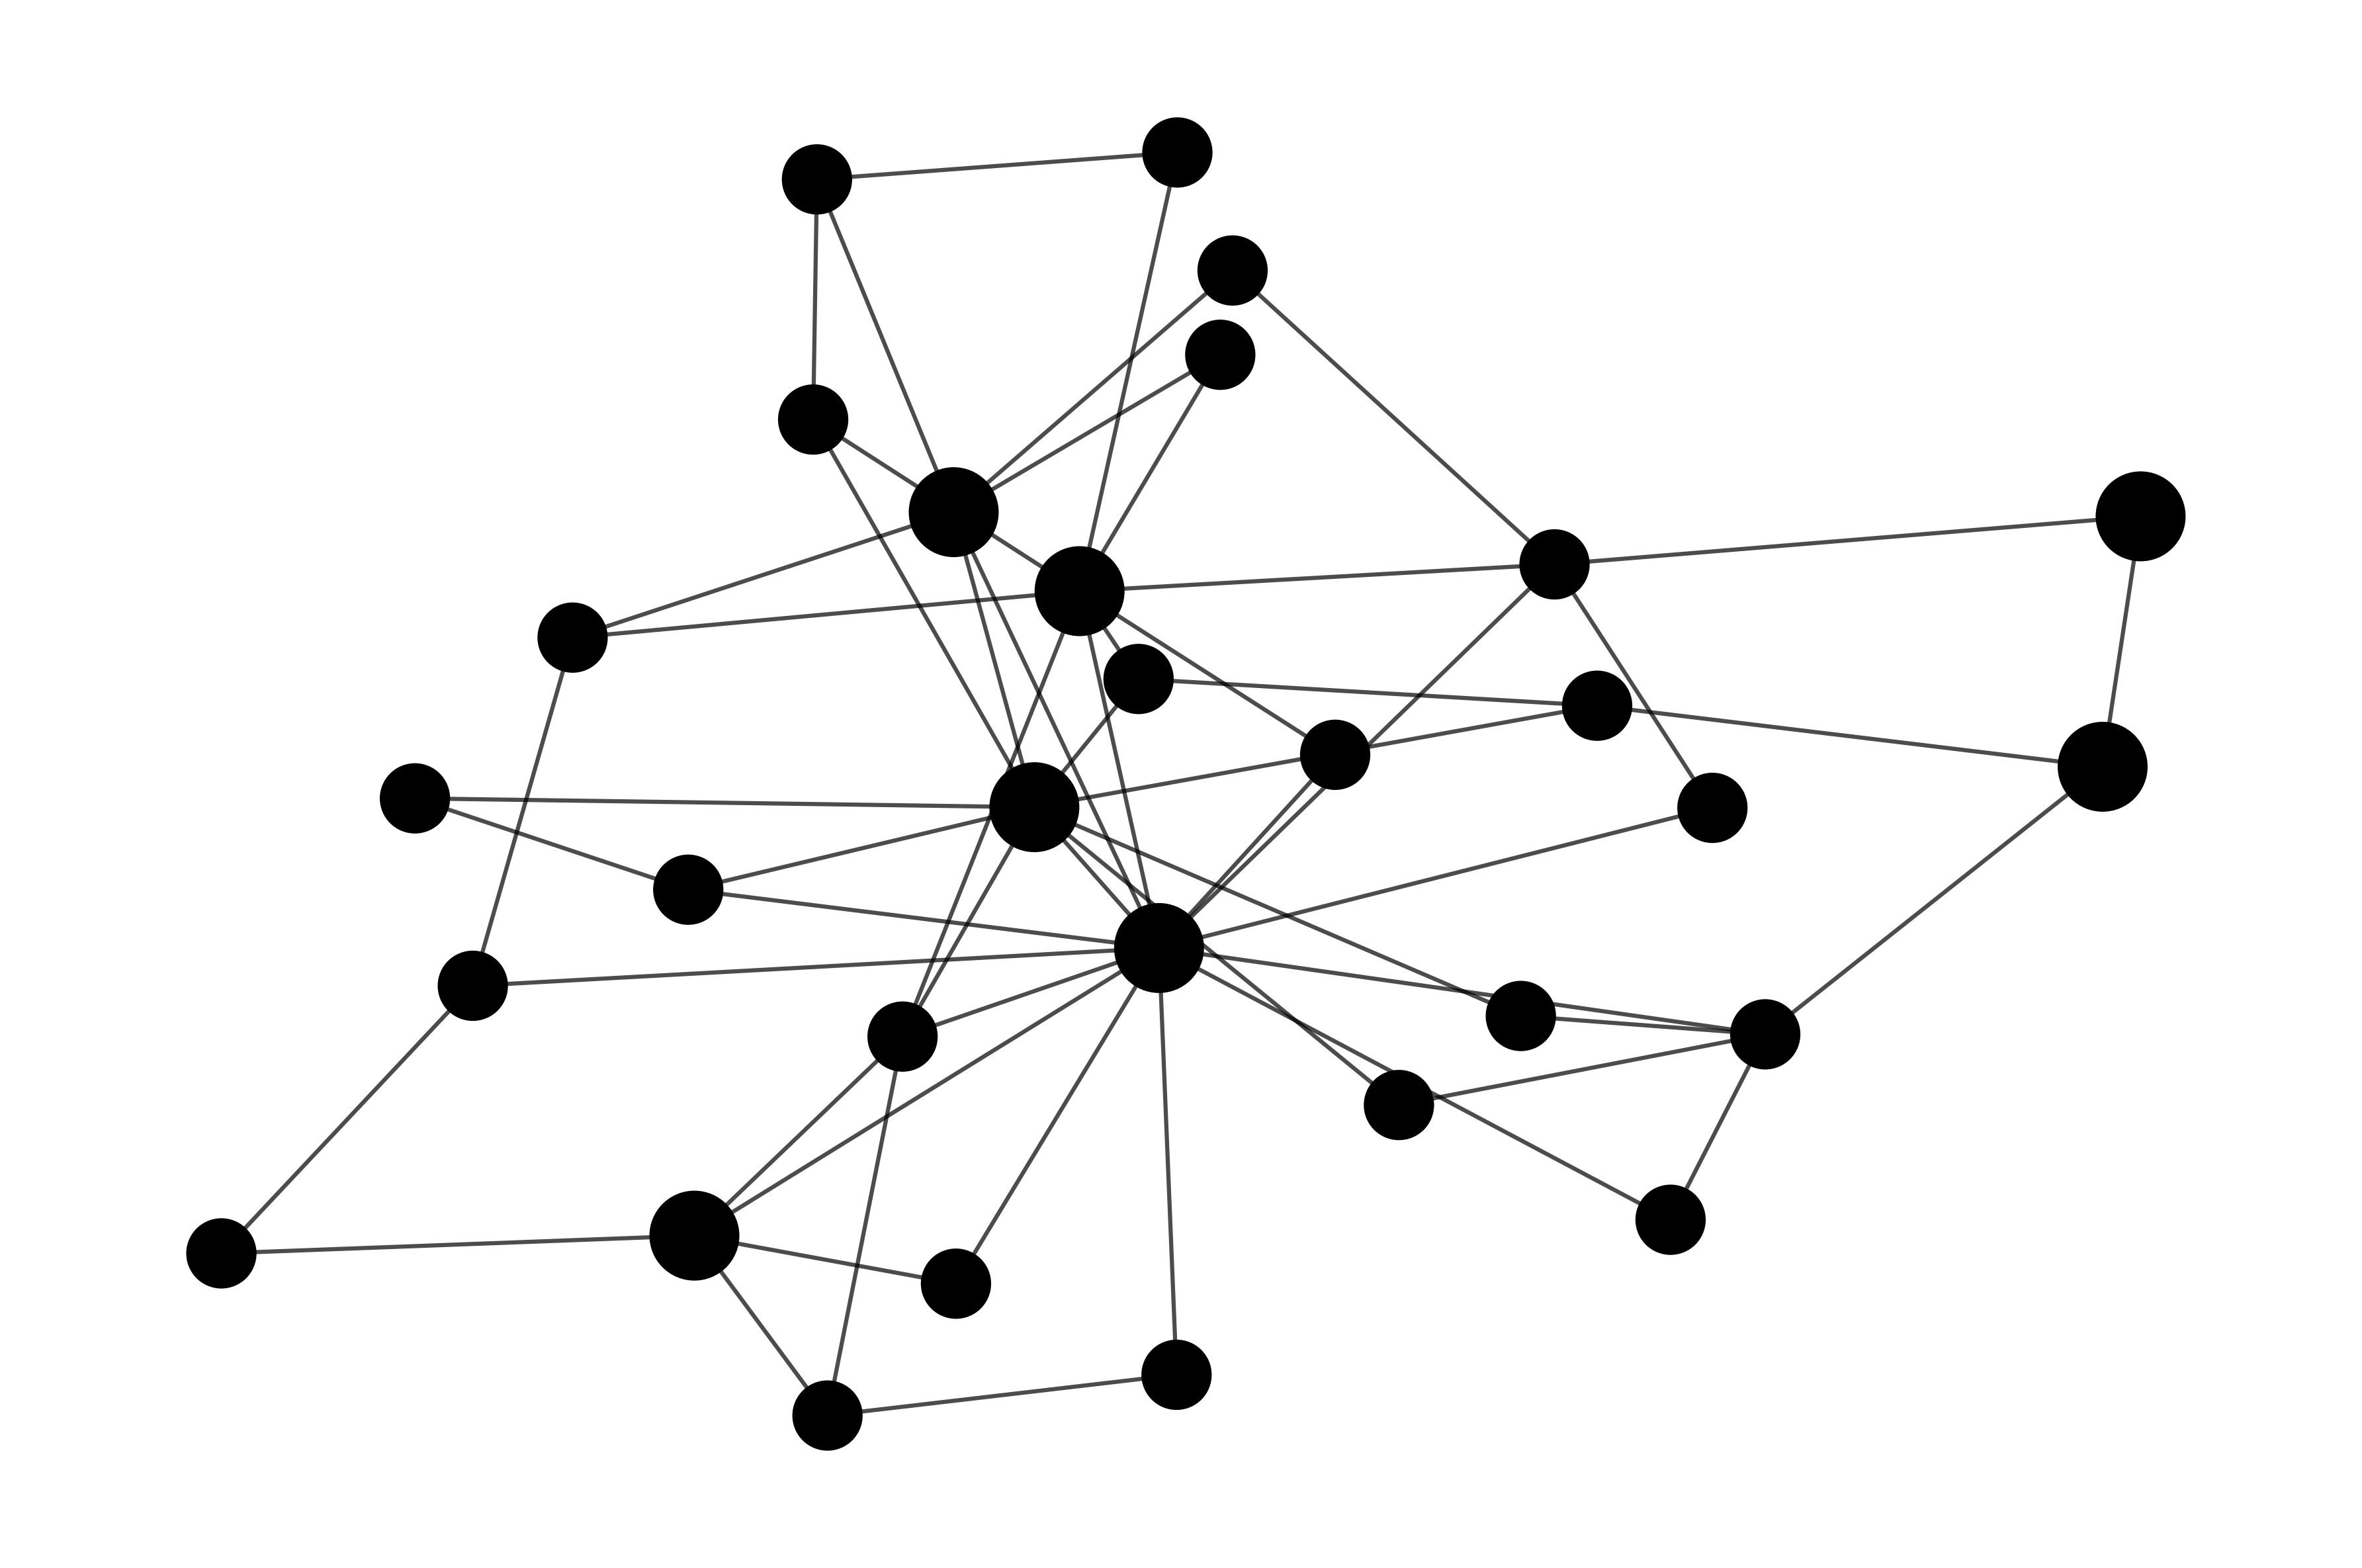
\includegraphics[width=0.6\textwidth]{assets/test_data/scalefree.png}
    \caption{Przykładowa realizacja grafu Barabási--Albert z widocznymi hubami}
    \label{fig:BA}
\end{figure}

Parametrem wejściowym modelu Barabási--Albert jest przede wszystkim $n$ - docelowa liczba węzłów w grafie - oraz $m$ - liczba krawędzi, jakie dodaje każdy nowy węzeł. Procedura generowania rozpoczyna się od małego grafu startowego (np. klika złożona z $m$ wierzchołków, aby zapewnić początkową spójność). Następnie dodaje się kolejno nowe wierzchołki; każdy nowy węzeł łączy się z $m$ już istniejącymi wierzchołkami, przy czym prawdopodobieństwo połączenia z danym istniejącym węzłem jest proporcjonalne do jego bieżącego stopnia (tzw. reguła preferencyjnego łączenia, ang. preferential attachment). Mechanizm preferencyjnego przyłączania zwiększa prawdopodobieństwo dalszego wzrostu stopnia wierzchołków o wysokiej liczbie połączeń, czyli wierzchołki, które zyskały wiele połączeń na wcześniejszych etapach, mają większą szansę zdobyć kolejne połączenia, co prowadzi do wykładniczego rozkładu stopni wierzchołków.

Motywacją użycia modelu BA było odzwierciedlenie w danych testowych właściwości często spotykanej w sieciach społecznościowych i sieciach informacji - silnego zróżnicowania w stopniach węzłów. Dzięki grafom BA można przetestować algorytmy pod kątem radzenia sobie z obecnością hubów oraz z rozkładem stopni o ciężkim ogonie (ang. heavy-tailed distribution). Pojęcie ciężkiego ogona oznacza, że prawdopodobieństwo wystąpienia wierzchołków o bardzo dużym stopniu maleje stosunkowo wolno - w efekcie w sieci, obok wielu węzłów o niskim stopniu, pojawia się również pewna liczba hubów o ekstremalnie wysokim stopniu. Zjawisko to odróżnia sieci bezskalowe od np. grafów ER, w których prawdopodobieństwo pojawienia się węzłów o bardzo dużej liczbie sąsiadów jest znikome.

Grafy generowane modelem BA mają z reguły jedną składową spójności. Przy założeniu, że graf początkowy jest spójny i $m \ge 1$, każdy nowy wierzchołek dołącza do istniejącej struktury, więc sieć pozostaje spójna, a średni stopień w takim grafie wynosi około $2m$. Stąd gęstość grafu BA maleje wraz ze wzrostem $n$. Dla dużych grafów jest ona rzędu $\frac{2m}{n}$, co oznacza, że grafy te są rzadkie. W przeciwieństwie do modelu ER, współczynnik skupienia grafów BA nie jest determinowany przez pojedynczy parametr w oczywisty sposób - klasyczny model BA generuje sieci o stosunkowo niskim średnim współczynnikiem klasteryzacji (niższym niż obserwowany w rzeczywistych sieciach społecznościowych), ponieważ nowe połączenia tworzone są głównie z hubami, co sprzyja tworzeniu gwiazd zamiast trójkątów. Istnieją modyfikacje modelu BA dodające mechanizmy triadycznego dosłączania, które zwiększają współczynnik klasteryzacji - jednak w czystej postaci model BA zazwyczaj skutkuje średnim współczynnikiem skupienia malejącym wraz z rozmiarem grafu. Niemniej jednak, nawet przy relatywnie niskim współczynniku klasteryzacji, grafy BA zachowują własność małych średnich odległości. Powyższe cechy sprawiają, że grafy BA stanowią przydatny model testowy - oddają one istnienie hubów i krótkich odległości jak w wielu sieciach społecznościowych, choć nie odwzorowują silnego grupowania lokalnego.

\subsection{Model Watts--Strogatz - graf małego świata}
Trzecim fundamentalnym modelem wykorzystanym w pracy jest model Watts--Strogatz (WS), opisany przez Wattsa i Strogatza w 1998 roku~\cite{Watts1998}. Umożliwia on generowanie grafów małego świata (small-world networks), które łączą w sobie dwie istotne cechy: wysoki współczynnik skupienia (podobny do obserwowanego w sieciach regularnych) oraz niską średnią odległość (podobnie jak w grafach losowych). Model ten odzwierciedla fakt, że w sieciach społecznościowych często występują silnie zżyte grupy znajomych, a jednocześnie dowolne dwie osoby są połączone relatywnie krótką ścieżką znajomości.

Generacja grafu WS wymaga dostarczenia mu trzech parametrów: liczby wierzchołków, stopnia każdego wierzchołka w początkowej regularnej strukturze oraz prawdopodobieństwa istnienia krawędzi. Procedura rozpoczyna się od utworzenia grafu regularnego, gdzie każdy wierzchołek jest połączony z $k$ najbliższymi sąsiadami w cyklu (tj. tworzymy cykl z $n$ węzłów, a następnie każdy węzeł łączymy z $\frac{k}{2}$ następnymi i $\frac{k}{2}$ poprzednimi na cyklu, zakładając dla uproszczenia, że $k$ jest parzyste). Tak powstała sieć charakteryzuje się wysokim współczynnikiem klasteryzacji - węzły sąsiadujące na cyklu tworzą małe kliki.
Jednocześnie początkowa średnia odległość jest stosunkowo duża, bo graf tuż przed modyfikacją krawędzi ma strukturę cyklu, więc dystans między węzłami oddalonymi na cyklu jest znaczny. Na rys.~\ref{fig:WS} zilustrowano przykładową realizację grafu Watts--Strogatz, w której widoczne są opisane wyżej właściwości.

\begin{figure}[h]
    \centering
    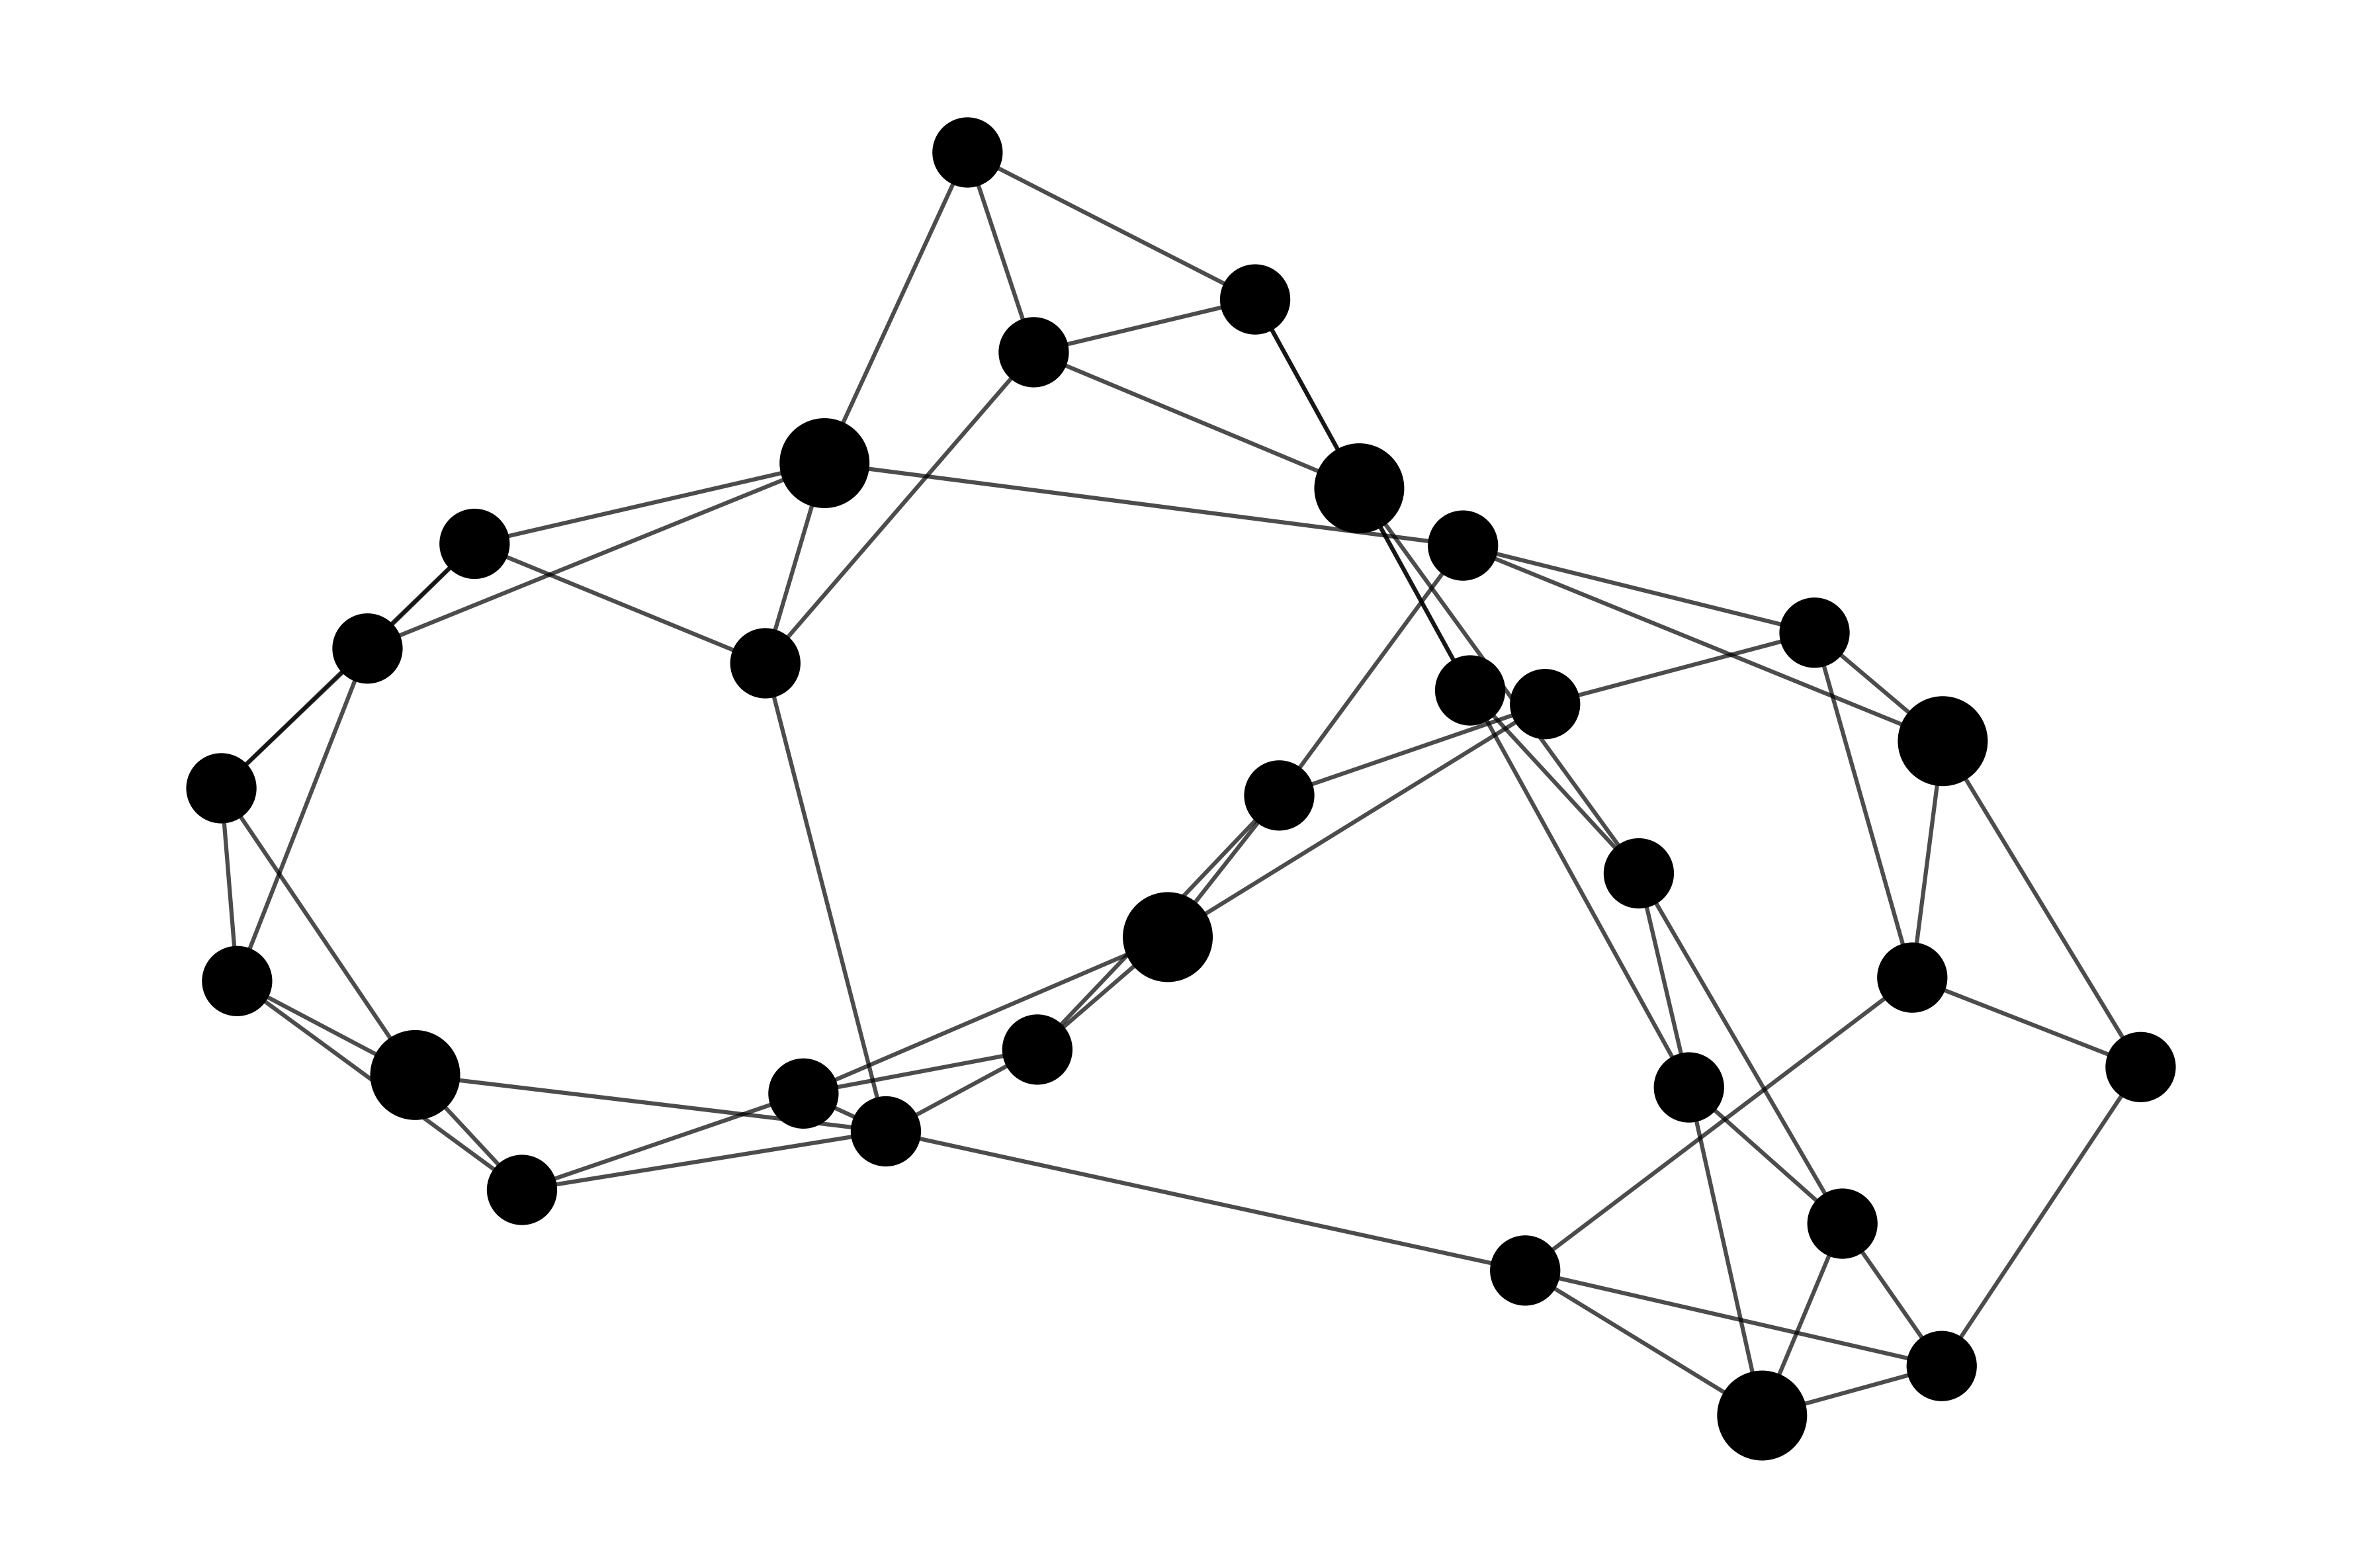
\includegraphics[width=0.65\textwidth]{assets/test_data/smallworld.png}
    \caption{Przykładowa realizacja grafu Watts--Strogatz, w której widoczne są lokalne kliki oraz losowe połączenia długodystansowe skracające średnie odległości}
    \label{fig:WS}
\end{figure}

Następnie, w modelu WS wprowadza się losowe przepięcia. Dla każdej krawędzi łączącej węzeł z jednym z $\frac{k}{2}$ najbliższych sąsiadów w cyklu. Dokonuje się, z prawdopodobieństwem $p$, przepięcia jednego końca tej krawędzi do losowo wybranego innego wierzchołka. Przepięcie polega na usunięciu oryginalnej krawędzi i dodaniu nowej krawędzi łączącej dany węzeł z innym losowym węzłem. W wyniku tych losowych przepięć, przy zachowaniu większości lokalnych połączeń cyklu, otrzymujemy graf, który dla małych $p$ wciąż charakteryzuje się wysokim współczynnikiem klasteryzacji, ale jednocześnie kilka losowych połączeń długodystansowych znacząco skraca średnie odległości w sieci. 
Dla umiarkowanych wartości $p$ (np. $p \approx 0.01$ czy $0.1$) sieć uzyskuje bardzo małą średnią odległość - zbliżoną do grafów losowych - podczas gdy współczynnik klasteryzacji pozostaje o rząd wielkości wyższy niż w grafie Erdős--Rényi o porównywalnej gęstości.

W kontekście modelowania sieci społecznościowych, generator dla modelu WS dodano w celu odzwierciedlenia właściwości, których brakuje modelowi BA - mianowicie wysokiego lokalnego współczynnika klasteryzacji. Sieci społecznościowe cechują się tym, że znajomi często znają się nawzajem, tworząc kliki znajomych. Model WS pozwala symulować taką sytuację i sprawdzić, jak algorytmy radzą sobie np. z wykrywaniem społeczności czy zjawisk rozprzestrzeniania się informacji w warunkach silnego grupowania. Parametr $k$ decyduje o początkowej gęstości połączeń lokalnych - większe $k$ to więcej krawędzi lokalnych (każdy węzeł ma początkowo $k$ sąsiadów), a zatem wyjściowo wyższy współczynnik klasteryzacji i gęstość. Parametr $p$ kontroluje losowość grafu. 
Dla $p=0$ otrzymujemy graf regularny, natomiast dla $p=1$ graf staje się w dużej mierze losowy. 
W praktycznych zastosowaniach szczególnie interesujący jest zakres wartości $p$ pomiędzy 0 a 1, w którym sieć łączy wysoki współczynnik klasteryzacji z niewielką średnią odległością między wierzchołkami.


Grafy WS generowane do testów miały parametry dobrane w taki sposób, aby możliwie dobrze odwzorowywać cechy typowe dla niedużych sieci społecznościowych. Uzyskiwane w ten sposób sieci charakteryzowały się relatywnie niską gęstością, ale jednocześnie wysokim współczynnikiem klasteryzacji, znacznie przewyższającym wartości obserwowane w losowych grafach ER o podobnej gęstości. Dzięki temu w grafach WS obecne są realistyczne zgrupowania lokalne, odpowiadające typowym kręgom znajomych w sieciach społecznościowych. Co istotne, sieci te z reguły pozostają spójne - niemal wszystkie wierzchołki należą do jednej dużej składowej spójności, a ewentualne izolowane węzły pojawiają się jedynie sporadycznie przy skrajnych ustawieniach parametrów. Taka struktura sprawia, że model WS stanowi dobre środowisko testowe.

\section{Grafy rzeczywiste}
Drugim zestawem danych testowych są rzeczywiste grafy pochodzące z sieci społecznościowej Facebook,
a dokładniej zbiór Facebook Ego Network udostępniony w ramach Stanford Network Analysis Project (SNAP)~\cite{snapnets}.
Dane te zostały zebrane w 2012 roku przez J. McAuley i J. Leskovca z Uniwersytetu Stanforda w ramach badań nad automatycznym wykrywaniem kręgów społecznościowych~\cite{McAuley2012}. Zbiór zawiera dziesięć tzw. ego-sieci - sieci ego-centrycznych poszczególnych użytkowników Facebooka, pozyskane za zgodą uczestników przy użyciu dedykowanej aplikacji badawczej działającej w ramach platformy Facebook. Ego-sieć to sieć społeczna z perspektywy pojedynczego użytkownika zwanego ego - węzłami są ego oraz wszystkie jego bezpośrednie znajome osoby, zaś krawędzie reprezentują relacje znajomości pomiędzy tymi znajomymi. W udostępnionych danych każda z dziesięciu sieci odpowiada innemu użytkownikowi i zawiera wyłącznie jego znajomych oraz powiązania między nimi. Węzeł ego nie jest jawnie ujęty jako wierzchołek w grafie i można go traktować jako ukrytą centralną jednostkę łączącą wszystkich znajomych. Innymi słowy, graf zapisany w pliku \verb|X.edges| dotyczy tylko znajomych użytkownika $X$ i relacji między nimi - sam $X$ nie pojawia się w pliku jako węzeł.

\subsection{Struktura danych}

Każda ego-sieć udostępnione przez SNAP zapisana jest w osobnych plikach tekstowych, których nazwa odpowiada identyfikatorowi \textit{ego} (np. \verb|0.edges|, \verb|0.circles|, \verb|0.feat|, \verb|0.egofeat| dla \textit{ego} o ID=0). Struktura danych jest następująca:

\textbf{Plik .edges} - lista krawędzi w grafie znajomych danego ego. Każdy wiersz zawiera dwie liczby - identyfikatory dwóch różnych znajomych ego, między którymi istnieje relacja koleżeńska. Krawędzie te są nieskierowane. Ważną cechą jest to, że plik \verb|.edges| nie zawiera połączeń od ego do jego znajomych - wierzchołek ego w ogóle nie występuje w tym pliku. Oznacza to, że rzeczywista sieć ego (gdyby uwzględnić w niej węzeł ego) miałaby dodatkowo krawędź łączącą ego z każdym z pojawiających się znajomych, jednak tych połączeń tutaj nie zapisano (są one domyślne - zakładamy, że ego jest połączone ze wszystkimi swoimi znajomymi). Pominięcie węzła ego jest zabiegiem celowym, pozwalającym skupić się na relacjach wewnątrz kręgów znajomych. Konsekwencją tego jest często podział grafu znajomych na kilka składowych - jeśli ego ma różne grupy znajomych wzajemnie się nieznających, to w pliku \verb|.edges| każda taka grupa stanowi osobną składową spójności. Przykładowo, w ego-sieci \verb|0.edges| znajomi tworzą 5 odrębnych składowych spójności. Oznacza to, że użytkownik o ID 0 miał około pięć niezależnych grup znajomych niepowiązanych ze sobą - dopiero poprzez jego osobę stawały się one pośrednio połączone.

\textbf{Plik .circles} - zestaw kręgów znajomych zdefiniowanych przez użytkownika. Każdy wiersz pliku reprezentuje jeden krąg towarzyski. Wiersz rozpoczyna się od nazwy kręgu - jednak w udostępnionych danych nazwy te zostały zanonimizowane lub pominięte, więc w praktyce każdy wiersz zaczyna się od identyfikatora kręgu albo pustej nazwy, po czym następuje lista ID użytkowników należących do tego kręgu. Kręgi mogą częściowo się pokrywać i nie muszą stanowić rozłącznych społeczności w sensie grafu - są to raczej dodatkowe metadane od ego, opisujące jak kategoryzuje on swoich znajomych. Informacje te mogą być cenne pomocniczo, np. w oryginalnej pracy McAuley'ego i Leskovca posłużyły do oceny algorytmów automatycznie wykrywających społeczności~\cite{McAuley2012}.

\textbf{Plik .feat} - macierz cech atrybutów przypisanych do znajomych ego. Każdy wiersz odpowiada jednemu znajomemu i zawiera wektor wartości cech tej osoby. Cechy te mogą obejmować informacje z profilu Facebooka (np. miejsce pracy, szkoła, zainteresowania itp.). W udostępnionym zbiorze wartości atrybutów zostały zanonimizowane - nie znamy dokładnego znaczenia poszczególnych cech, jedynie ich binarne wartości (1 - użytkownik posiada daną cechę, 0 - nie posiada). Istnieje także plik \verb|.featnames| zawierający oryginalne nazwy cech, ale w przypadku Facebooka nazwy te również zostały zanonimizowane (np. zamiast "szkoła: Uniwersytet Stanford" pojawia się anonimowa cecha 57). W niniejszej pracy dane atrybutów nie były wykorzystywane przez algorytmy i skupiono się tylko na strukturze grafów.

\textbf{Plik .egofeat} - wektor cech centralnego użytkownika, w tym samym formacie co pojedynczy wiersz pliku \verb|.feat|, odnoszący się jednak do ego. Pozwala to porównać cechy ego z cechami jego znajomych. W kontekście naszych badań plik ten również nie był bezpośrednio wykorzystywany, poza podstawową walidacją danych.

W eksperymentach wykorzystano wszystkie dziesięć ego-sieci dostępnych w zbiorze SNAP. Liczba węzłów (po pominięciu centralnego ego) wynosiła odpowiednio 53, 62, 151, 169, 225, 334, 535, 748, 787 oraz 1035. Tak szeroki zestaw umożliwił ocenę algorytmów zarówno na niewielkich, jak i ponadtysięcznych grafach, w których różnice w gęstości i strukturze społeczności są wyraźnie widoczne.

\subsection{Szczegółowy opis danych ze zbioru SNAP}
W badanym zbiorze występują zarówno niewielkie sieci liczące poniżej setki węzłów (np. ID 3980: 53 wierzchołki, 252 krawędzie), jak i bardzo duże instancje przekraczające tysiąc węzłów (ID 0: 1035 wierzchołków, ponad 26\,000 krawędzi). Ogólnie rzecz biorąc, większa liczba znajomych oznacza większe zróżnicowanie strukturalne: część ego-sieci składa się z kilku gęstych społeczności, podczas gdy inne są rozproszone i tworzą liczne składowe. Sumarycznie wszystkie dziesięć ego-sieci obejmuje 4039 unikalnych wierzchołków oraz 88\,234 krawędzie \cite{McAuley2012}, co dobrze oddaje skalę i złożoność sieci osobistych kontaktów.

Jak wspomniano, z powodu braku węzła ego w grafie znajomych większość ego-sieci dzieli się na więcej niż jedną składową spójności. W praktyce zazwyczaj istnieje jedna dominująca składowa, zawierająca największą grupę wzajemnie powiązanych znajomych, oraz kilka mniejszych składowych (np. dwu- lub kilkuosobowych grup) odpowiadających odizolowanym kręgom towarzyskim. Dla przykładu, sieć \verb|107.edges| okazała się całkowicie spójna - wszyscy znajomi użytkownika 107 tworzyli jeden graf spójny. Natomiast sieć \verb|0.edges| miała 5 składowych - co już sygnalizowano wcześniej. Wśród naszych analizowanych sieci: sieć \verb|686.edges| jest spójna, sieć \verb|414.edges| dzieli się na 2 składowe, sieć \verb|698.edges| na 3, a sieć \verb|3980.edges| na 4 składowe. Zwykle największa składowa obejmuje zdecydowaną większość wierzchołków. Taka struktura wskazuje na obecność jednego głównego kręgu znajomych, uzupełnionego kilkoma mniejszymi grupami znajomości niepowiązanych z resztą.

Ego-sieci Facebooka cechują się na ogół wysokim współczynnikiem klasteryzacji, co zgodne jest z intuicją - znajomi konkretnej osoby często znają się nawzajem. W literaturze podaje się, że globalny współczynnik klasteryzacji dla całego grafu Facebooka jest stosunkowo niski~\cite{Ugander2011}. W obrębie pojedynczej ego-sieci, gdzie wszyscy rozważani ludzie są znajomymi jednego ego, współczynnik skupienia jest znacznie wyższy. Dla połączonej sieci 10 ego (4039 węzłów) średni współczynnik klasteryzacji wynosił aż 0.6055, co oznacza, że dwaj losowo wybrani znajomi danego ego mieli ponad 60\% szans, by również być znajomymi między sobą. W naszych mniejszych sieciach wartości te różnią się w zależności od sieci, ale zwykle mieszczą się w przedziale 0.5-0.6 dla największej składowej (mniejsze składowe, np. dwuosobowe, mają współczynnik klasteryzacji równy 0 lub nieokreślony). Wysoki średni współczynnik skupienia potwierdza istnienie silnych lokalnych powiązań - w grafie występuje wiele trójkątów (grup znajomych, z których każdy zna pozostałych). Przykładowo, jeśli ego posiada grupę bliskich przyjaciół ze szkoły, to prawdopodobne jest, że większość z nich zna się nawzajem, tworząc pełne podgrafy (kliki) o dużym współczynniku klasteryzacji.

Gęstość, rozumiana jako stosunek liczby istniejących krawędzi do maksymalnej liczby krawędzi możliwej między daną liczbą wierzchołków, w ego-sieciach Facebooka jest stosunkowo niska w kategoriach bezwzględnych (co wynika z faktu, że sieci społecznościowe z natury są rzadkie). Typowe wartości w badanym zbiorze mieszczą się od kilku do kilkunastu procent: największe sieci (powyżej 700 węzłów) osiągają gęstości około 0.05, natomiast mniejsze instancje (53 i 62 węzły) przekraczają 0.15 dzięki bardziej lokalnym połączeniom. W porównaniu do grafów losowych o podobnej skali ego-sieci mają wyższy współczynnik klasteryzacji (krawędzie nie są rozłożone przypadkowo, lecz skoncentrowane wewnątrz grup), natomiast same wartości gęstości pozostają rzędu kilku procent. Ta rzadka natura sieci społecznościowych jest istotna z punktu widzenia testowanych algorytmów, gdyż wiele z nich ma złożoności silnie zależne od liczby krawędzi (np. operacje przeszukiwania grafu lub znajdowania struktur klikowych mogą być szybsze w grafach rzadszych).
